\documentclass[10pt]{beamer}

\usetheme[progressbar=frametitle]{metropolis}
\usepackage{appendixnumberbeamer}

\usepackage{booktabs}
\usepackage[scale=2]{ccicons}
\usepackage[utf8]{inputenc}
\usepackage{graphicx}
\usepackage[]{media9}

\usepackage{pgfplots}
\usepgfplotslibrary{dateplot}

\usepackage{xspace}
\newcommand{\themename}{\textbf{\textsc{metropolis}}\xspace}
\newcommand\tab[1][0.6cm]{\hspace*{#1}}
\newcommand\supertab[1][2.9cm]{\hspace*{#1}}
\title{Trenzas y criptografía}
 %\date{\today}
\date{}
\author{Lucía Asencio}
%\institute{Center for modern beamer themes}
% \titlegraphic{\hfill\includegraphics[height=1.5cm]{logo.pdf}}

\begin{document}

\maketitle

%\begin{frame}{Table of contents}
 % \setbeamertemplate{section in toc}[sections numbered]
  %\tableofcontents[hideallsubsections]
%\end{frame}

\section{Grupos}

\begin{frame}[fragile]{¿Qué es un grupo?}
\begin{center}
		\includegraphics[width=225pt]{color.png}
\end{center}
\end{frame}	

\begin{frame}[fragile]{¿Qué es un grupo?}
Tendremos:
  \begin{itemize}
  	\item Un conjunto de \alert{\textbf{elementos}},
  	\item Una \alert{\textbf{operación}}, 
  	\item Cada elemento tendrá su \alert{\textbf{inverso}} respecto a la operación,
  	\item Unos pocos \alert{\textbf{generadores}} de todos los elementos
  
  \end{itemize}
\end{frame}
\begin{frame}[fragile]{Ejemplos feítos}
  	\begin{columns}[T,onlytextwidth]
		\column{0.5\textwidth}
		$\mathbb{(Z, +)}$
		\begin{description}
			\item[Elementos] $-\infty\ldots0,1,2\ldots\infty $
			\item[Operación] $n_1 + n_2$
			\item[Inversos] $1 \rightarrow -1, \newline2 \rightarrow -2, \newline  \vdots \newline n \rightarrow -n$
		\end{description}
		
		\column{0.55\textwidth}
		$GL_n\mathbb{(R)}$
		\begin{description}
			\item[Elementos] $\mathcal{M}$ matrices invertibles
			\item[Operación] $\mathcal{M}_1 \cdot \mathcal{M}_2$ 
			\item[Inversos] $\mathcal{M} \rightarrow \mathcal{M}^{-1}$
		\end{description}
		
		
		
	\end{columns}
  
\end{frame}

\section{Trenzas}

\begin{frame}{¿Qué son?}
	Trenzas cortas, trenzas largas, sencillas, complejas... \newline 

	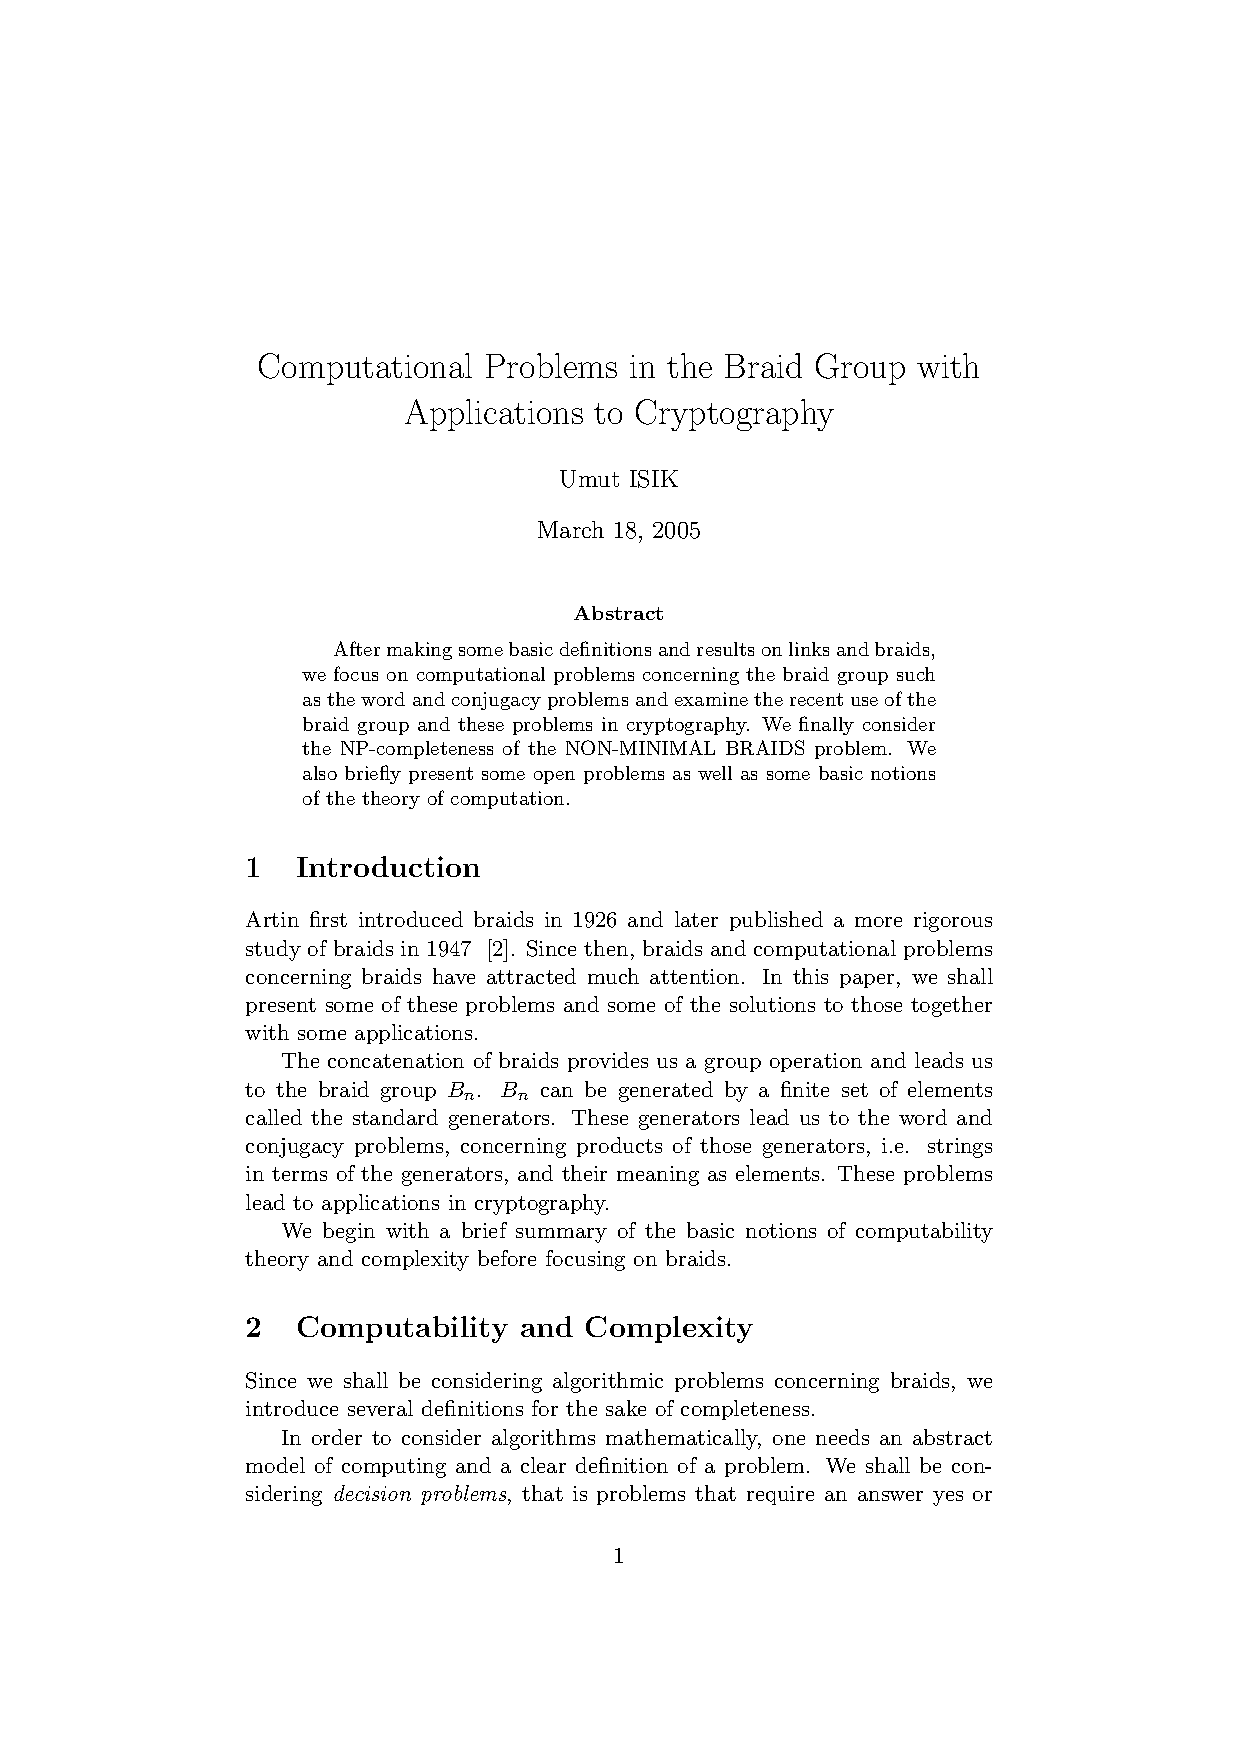
\includegraphics[width=300pt]{braids.jpg}
	
\end{frame}


\begin{frame}{Como grupo}
	\begin{description}
		\item[Elementos]  Todas las trenzas del mundo mundial 
		\item[Operación] ¡Concatenar!\newline $\sigma_1 \cdot \sigma_2 = \sigma_1\sigma_2
		\newline \sigma_1\cdot \sigma_2\cdot \sigma_1 = \sigma_1\sigma_2\sigma_1$
		\item[Inversos] Espejo
		\item[Generadores] Las mini-trenzas $\sigma_1, \sigma_2 \ldots \sigma_{n-1}$
		
	\end{description}
	\includegraphics[width=325pt]{gens.jpg}\newline
	$\tab \sigma_1$ \supertab $\sigma_2$ \supertab $\sigma_3 \tab\tab\tab\tab \sigma_4$
\end{frame}

\begin{frame}{Problemas}
	\begin{enumerate}
		\item ¿Cuándo dos trenzas son iguales?
		\item ¿Cuándo dos trenzas son conjugadas?
	\end{enumerate}
	%\metroset{block=fill}
	\begin{exampleblock}{Conjugación }
		\begin{itemize}
			\item 2 trenzas $a, b$ 
			\item Conjugar $a$ por $b = conjugar(a, b) = b\cdot a\cdot b^{-1} = c$ 
			\item Decimos que $a$ y $c$ están conjugadas
		\end{itemize}
	\end{exampleblock}
\end{frame}

\section{Criptografía}

\begin{frame}[fragile]{Protocolo de intercambio de claves}

\begin{columns}[T,onlytextwidth]
	\column{0.5\textwidth}
	
	\begin{center}
		\texttt{
			Alice $\rightarrow$ clave privada \textbf{$a$} \newline
			\tab $+$\newline
			Bob $\rightarrow$ clave privada \textbf{$b$} \newline
			\tab $+$\newline
			Alice y Bob comparten públicamente información  \textbf{$p$} \newline
			\tab$+$ \newline
			Mensajes A $\leftrightarrow$ B en canal inseguro \newline
			\tab$=$ \newline
			Clave secreta compartida entre Alice y Bob \newline}
	\end{center}
	
	\column{0.4\textwidth}
	\includegraphics[width=100pt]{dh.png}
	
	
	
\end{columns}



  
\end{frame}

\begin{frame}{Protocolo de intercambio de claves... con trenzas}
	Trenzas de 7 cuerdas ($\equiv$ multiplicar $\sigma_1, \sigma_2, \sigma_3 \ldots \sigma_6$ )
	\begin{description}
		\item[Comparten]  $p = \{\sigma_1, \sigma_2, \sigma_3\}$ 
		\item[K$^-$ Alice] $a = \sigma_1\sigma_2\sigma_1^{-1}\sigma_3$
		\item[K$^-$ Bob] $b = \sigma_3\sigma_2\sigma_1^{-1}\sigma_2^{-1}$		
		\item[Alice $\rightarrow$ Bob] $\{a\sigma_1a^{-1}, a\sigma_2a^{-1}, a\sigma_3a^{-1}\}$
		\item[Bob $\rightarrow$ Alice] $\{b\sigma_1b^{-1}, b\sigma_2b^{-1}, b\sigma_3b^{-1}\}$
		\item[Secreto ] $aba^{-1}b^{-1}$
	\end{description}
\end{frame}

\begin{frame}{¿Y ahora?}

	 The minimal braid problem? \newline
	 The square-root problem? \newline
	 E-multiplication?
	
	
\end{frame}

\end{document}
